\section{Introducción}
%Una línea de transmisión es un medio físico por el cual se propaga una señal eléctrica desde un emisor a un receptor. En su forma más usual, consiste en dos hilos conductores paralelos, llamada línea \textit{bifiliar}, o dos conductores cilíndricos concéntricos, lo que corresponde a una línea \textit{coaxial}. 

%Es posible modelar una línea de transmisión como un conjunto de elementos \textit{concentrados} o de elementos \textit{distribuidos}, según la relación existente entre las dimensiones del circuito y la longitud de onda de la señal. En un modelo de elementos concentrados, los componentes característicos de un circuito (como lo es la inductancia, capacitancia y resistencia) se encuentran localizados en una pequeña fracción del espacio (o de la línea?), la cual resulta despreciable respecto a la longitud de onda de la señal que se propaga.  Por otro lado, en un modelo de elementos distribuidos, los componentes se distribuyen de manera continua a lo largo de la línea, lo cual permite el estudio de señales con longitudes de onda comparable a las dimensiones del circuito. 

Una línea de transmisión es un medio físico por el cual se propaga una señal eléctrica desde un emisor a un receptor. A diferencia de un circuito eléctrico, el cual supone que las dimensiones físicas de la red son mucho menores que la longitud de onda que se propaga (modelo de elementos \textit{concentrados}), las líneas de transmisión se modelan como elementos \textit{distribuidos}, permitiendo el análisis de señales con longitud de onda comparable a las dimensiones del circuito. \cite{pozar2012}

En su forma más usual, una línea de transmisión consiste en un hilo conductor concéntrico a una lámina cilíndrica también conductora, llamada línea coaxial (Ver \autoref{fig:cable_coaxial}). La corriente que circula por el hilo conductor genera un campo magnético, el cual se modela como una inductancia $L$ en el circuito de la \autoref{fig:cable_coaxial_circuito}, debido a que el cable no es ideal, se le coloca una resistencia $R$ en serie. Por otro lado, entre el hilo conductor y la lámina cilíndrica existe una diferencia de potencial $V$, la cual puede modelarse como una capacitancia $C$ en paralelo a una conductancia $G$. La capacitancia representa el almacenamiento de energía del campo eléctrico existente entre ambos conductores, mientras que la conductancia simula las pérdidas asociadas a la conductividad del dieléctrico que las separa.

Un fenómeno análogo ocurre en la propagación de impulsos eléctricos a través de las neuronas, donde el axón actúa como una línea de transmisión. Como respuesta a un estímulo, las neuronas generan breves pulsos de voltaje que, al superar un determinado umbral, la membrana se despolariza generando un potencial de acción el cual se propaga a lo largo del axón. 

La membrana neuronal separa soluciones de diferentes concentraciones iónicas, lo que genera una diferencia de potencial de aproximádamente \SI{70}{\milli\volt} entre el interior y el exterior de la célula. Esta diferencia de potencial puede modelarse como una fem. Además, debido a la acumulación de iones con cargas opuestas entre ambos lados de la membrana, se introduce un capacitor el cual simula el almacenamiento de energía. Luego, la permeabilidad de la membrana al transporte de distintos iones puede representarse mediante una resistencia equivalente. De esta manera, es posible modelar la membrana neuronal a través de un circuito RC, donde la constante de tiempo $\tau$ determina el tiempo que tarda el potencial de la membrana en alcanzar un estado estacionario tras un estímulo.

Las analogías que se realizan entre distintos problemas físicos con líneas de transmisión son amplias, donde existen relaciones entre distintas magnitudes físicas cuyo comportamiento es el mismo. Por ejemplo, en un fluido viscoso newtoniano contenido en un recipiente que oscila, su movimiento está dado por el segundo problema de Stokes, que se reduce a una ecuación de difusión. De la misma manera que una escalera RC propaga una señal, la velocidad del fluido toma el papel del voltaje, la viscosidad representa la resistencia y la elasticidad del medio el capacitor \cite{Hayat2004StokesSP}.

\begin{figure}[H]
\centering
\begin{subfigure}{0.45\textwidth}
    \centering
    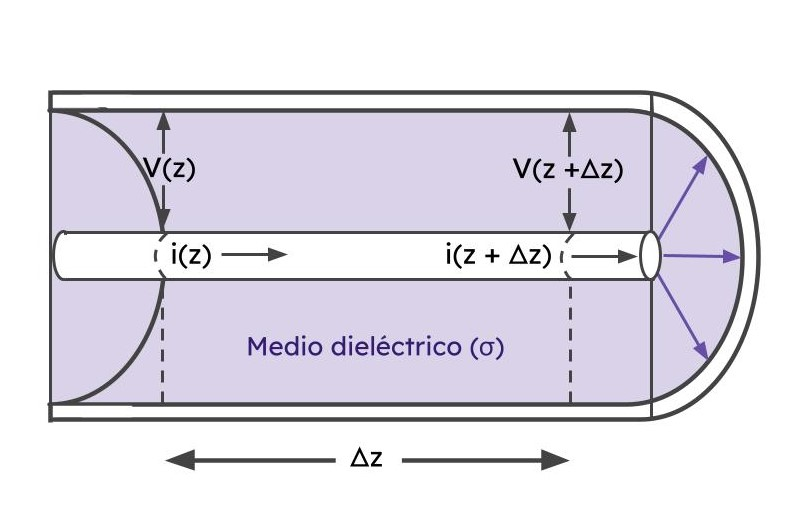
\includegraphics[width=\linewidth]{gráficos/cable coaxial.jpg}
    \caption{}
    \label{fig:cable_coaxial}
\end{subfigure}
\hfill
\begin{subfigure}{0.45\textwidth}
    \centering
    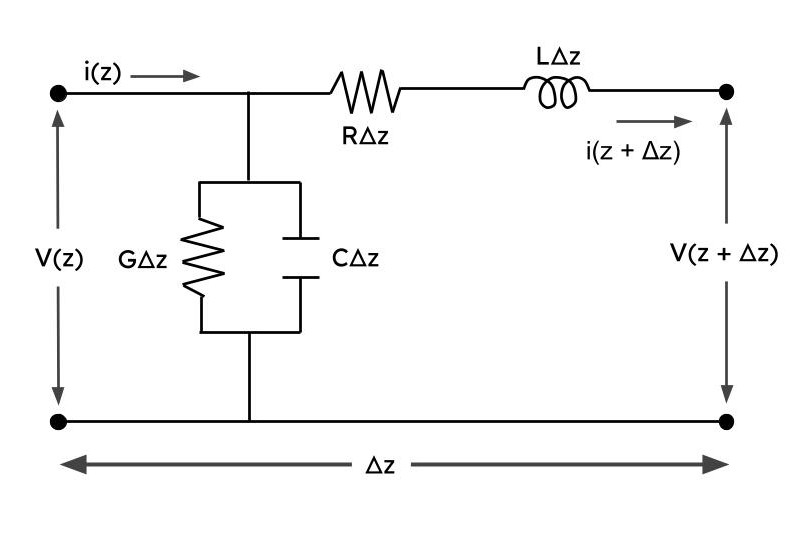
\includegraphics[width=\linewidth]{gráficos/circuito del telegrafista.jpg}
    \caption{}
    \label{fig:cable_coaxial_circuito}
\end{subfigure}
\caption{Diagrama de un cable coaxial (a) junto a su circuito equivalente (b).}
\label{fig:coaxial_comparación}
\end{figure}
Las tensiones y corrientes pueden variar tanto en magnitud como en fase a lo largo de la longitud de la línea, por lo que deben describirse como funciones de la posición. De esta manera, cada componente de la red eléctrica ($R$, $L$, $G$ y $C$) se define por unidad de longitud $\Delta z$, obteniendo una ecuación diferencial de segundo orden del potencial $V$ respecto a $z$  \cite{preston1991} para el circuito de la \autoref{fig:cable_coaxial_circuito} como

\begin{equation}
    \frac{\partial^2 V}{\partial z^2} = RGV + (RC + LG)\,\frac{\partial V}{\partial t} + LC\,\frac{\partial^2 V}{\partial t^2}
    \label{eq:difV}
\end{equation} 

En este experimento, se modeló un cable coaxial utilizando la ecuación del Telegrafista \eqref{eq:difV} y se estudió un modelo límite a bajas frecuencias como un circuito RC en escalera, con el fin de estudiar la propagación de señales eléctricas a través de la red. Además, se propagó un pulso cuadrado en un cable coaxial, estableciendo distintas impedancias en uno de sus extremos, con el fin de analizar la señal reflejada respecto a la incidente.